\begin{tikzpicture}
	\draw[orange, dashed] (1.4, 1.1) -- (12.15, 1.1);
	\draw[orange, dashed] (1.4, 1.1) -- (1.4, 3.1);
	\draw[orange, dashed] (12.15, 1.1) -- (12.15, 3.1);
	\node[orange] at (6.8, 1.4) {$z(t) = A \cdot e^{\mathrm{j} \varphi} \cdot e^{\mathrm{j} \omega t}$};
	\node[orange] at (1.4, 1.1) {\textbullet};
	\node[orange] at (12.15, 1.1) {\textbullet};
	\draw[orange, dashed] (6.1, 3.8) -- (8.2, 3.8);
	\draw[orange, dashed] (6.1, 3.1) -- (6.1, 3.8);
	\draw[orange, dashed] (8.2, 3.1) -- (8.2, 3.8);
	\node[orange] at (7.2, 4.1) {$z(G) = A \cdot e^{\mathrm{j}\varphi}$};
	\node[orange] at (6.1, 3.8) {\textbullet};
	\node[orange] at (8.2, 3.8) {\textbullet};
	\scalebox{1}{\begin{tikzpicture}
	%\draw[help lines] (0,0) grid (6,4);
	\begin{axis}[axis lines=middle, axis equal, grid=both, xlabel = $\operatorname{Re}$, ylabel = $\operatorname{Im}$]
		\draw[black!70] ([shift=(60:1cm)]180, 75) arc(0:360:2.58cm);
		\addplot[->, blue, very thick] coordinates{(0, 0) (-0.71, -0.71)}  node[sloped, above, blue] {$A$};
		\addplot[->, blue, very thick] coordinates{(0, 0) (0.94, 0.25)}  node[sloped, above, blue] {$A$};
		\addplot[->, dashed, white] coordinates{(0, 0) (1, -1.1)}; % for axis-scaling
		\addplot[->, dashed, white] coordinates{(0, 0) (-1, 1.1)}; % for axis-scaling
	\end{axis}
\end{tikzpicture}}
	\scalebox{1}{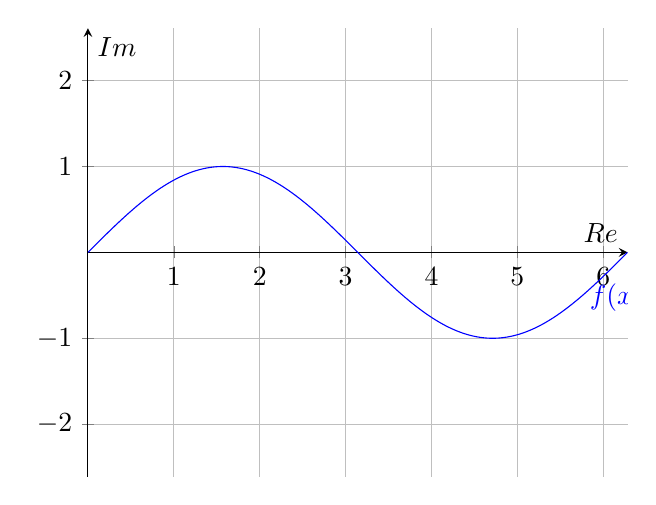
\begin{tikzpicture}
	%\draw[help lines] (0,0) grid (6,4);
	\begin{axis}[axis lines=middle, axis equal, grid=both, xlabel = $\operatorname{Re}$, ylabel = $\operatorname{Im}$]
		\addplot[domain=0:2*pi,samples=200,blue]{sin(deg(x))}node[right,pos=0.9]{$f(x)=\sin x$};
	\end{axis}
\end{tikzpicture}}
\end{tikzpicture}